\documentclass{beamer}
\usepackage{tikz}
\usepackage{amsmath}
\usepackage{amssymb}

\usetheme{Madrid}
\usecolortheme{beaver}

% Define a command for the introduction of logical symbols
\newcommand{\newlogicalsymbol}[2]{
\textbf{#1}: #2
}

\title{Argument Evaluation}
\subtitle{Principles of Logic and Critical Thinking}
\author{Instructor Name}
\date{\today}

\begin{document}

\begin{frame}
\titlepage
\end{frame}

\begin{frame}
\frametitle{1. What Makes a Good Argument? An Overview}
\begin{itemize}
\item An \textbf{argument} is a set of statements where some (premises) are offered to support another (conclusion).
\item Good arguments require both \textbf{logical validity} and \textbf{factual truth}.
\item Arguments are fundamental to critical thinking and rational discourse.
\item Evaluating arguments helps us separate sound reasoning from flawed thinking.
\end{itemize}

\begin{block}{Two Central Questions in Argument Evaluation}
\begin{enumerate}
\item Do the premises adequately support the conclusion?
\item Are the premises actually true?
\end{enumerate}
\end{block}
\end{frame}

\begin{frame}
\frametitle{2. Review: Identifying Premises and Conclusions}
\begin{itemize}
\item \textbf{Premises} are statements offered as reasons or evidence to support a conclusion.
\item \textbf{Conclusions} are claims that follow from or are supported by premises.
\item Indicator words signal premises (because, since, given that) and conclusions (therefore, thus, hence).
\item Some arguments have implicit (unstated) premises or conclusions that need to be identified.
\end{itemize}

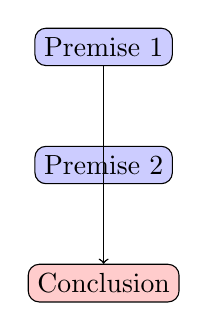
\begin{tikzpicture}[node distance=1.5cm]
\node (premise1) [draw, rectangle, rounded corners, fill=blue!20] {Premise 1};
\node (premise2) [draw, rectangle, rounded corners, fill=blue!20, below of=premise1] {Premise 2};
\node (conclusion) [draw, rectangle, rounded corners, fill=red!20, below of=premise2] {Conclusion};
\draw[->] (premise1) -- (conclusion);
\draw[->] (premise2) -- (conclusion);
\end{tikzpicture}
\end{frame}

\begin{frame}
\frametitle{3. Converting Arguments to Standard Form}
\begin{itemize}
\item \textbf{Standard form} arranges an argument with premises listed first and conclusion last.
\item Converting to standard form helps clarify the logical structure of an argument.
\item Each premise should be a single, clear statement with one main idea.
\item Number premises (P1, P2, etc.) and clearly mark the conclusion (C).
\end{itemize}

\begin{example}
Original: "Since it's raining and the streets are wet, you should take an umbrella."

Standard Form:
\begin{enumerate}
\item[P1:] It is raining.
\item[P2:] The streets are wet.
\item[C:] You should take an umbrella.
\end{enumerate}

\end{example}
\end{frame}

\begin{frame}
\frametitle{4. The Principle of Charity: Interpreting Arguments Fairly}
\begin{itemize}
\item The \textbf{principle of charity} requires interpreting arguments in their strongest possible form.
\item Charitable interpretation means finding the most reasonable interpretation of unclear statements.
\item We should focus on evaluating the substance rather than attacking weak expressions.
\item Avoiding "straw man" arguments shows intellectual honesty and strengthens our own reasoning.
\end{itemize}

\begin{alertblock}{Why Practice Charity?}
Applying the principle of charity:
\begin{itemize}
\item Demonstrates intellectual integrity
\item Leads to more productive discussions
\item Helps identify the strongest counterarguments
\item Prevents wasting time on superficial disagreements
\end{itemize}
\end{alertblock}
\end{frame}

\begin{frame}
\frametitle{5. Test \#1: Do the Premises Support the Conclusion?}
\begin{itemize}
\item This test examines the \textbf{logical relationship} between premises and conclusion.
\item We ask: "If all premises were true, would the conclusion necessarily or probably follow?"
\item This test focuses on the structure of the argument, not the content.
\item An argument can pass this test even if its premises are actually false.
\end{itemize}

\begin{table}
\scriptsize
\begin{tabular}{|l|l|}
\hline
\textbf{Strong Support} & \textbf{Weak Support} \\
\hline
Conclusion follows necessarily & Conclusion doesn't follow \\
Conclusion follows with high probability & Connection is tenuous \\
Logical structure is sound & Logical gaps exist \\
All relevant factors considered & Important factors missing \\
\hline
\end{tabular}
\end{table}
\end{frame}

\begin{frame}
\frametitle{6. Test \#2: Are the Premises Actually True?}
\begin{itemize}
\item This test examines the \textbf{factual accuracy} of each premise.
\item We must verify premises through observation, research, or established knowledge.
\item Some premises may be true in certain contexts but not in others.
\item Arguments with false premises can never be sound, even if logically valid.
\end{itemize}

\begin{block}{Methods to Verify Premises}
\begin{itemize}
\item Direct observation or experience
\item Reliable scientific evidence
\item Credible expert testimony
\item Logical necessity (e.g., mathematical truths)
\end{itemize}
\end{block}
\end{frame}

\begin{frame}
\frametitle{7. The Relationship Between Truth and Validity}
\begin{itemize}
\item \textbf{Validity} concerns the logical structure regardless of factual content.
\item \textbf{Truth} concerns the factual accuracy of individual statements.
\item A \textbf{sound argument} is both valid and has all true premises.
\item Validity + Truth = Soundness (the gold standard for arguments).
\end{itemize}

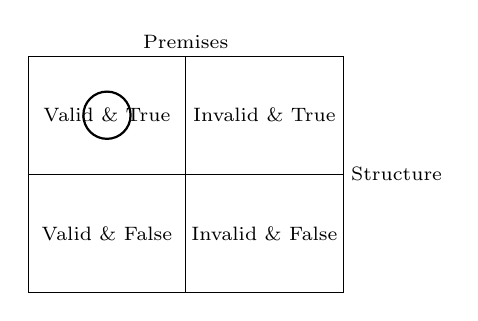
\begin{tikzpicture}
\scriptsize
\draw (0,0) rectangle (4,3);
\draw (0,1.5) -- (4,1.5);
\draw (2,0) -- (2,3);
\node at (1,2.25) {Valid \& True};
\node at (3,2.25) {Invalid \& True};
\node at (1,0.75) {Valid \& False};
\node at (3,0.75) {Invalid \& False};
\node[above] at (2,3) {Premises};
\node[right] at (4,1.5) {Structure};
\draw[thick, ->] (1,2.25) circle (0.3);
\end{tikzpicture}
\end{frame}

\begin{frame}
\frametitle{8. Common Mistakes in Argument Evaluation}
\begin{itemize}
\item \textbf{Conflating truth and validity}: An argument can be valid with false premises.
\item \textbf{Accepting weak support}: Assuming premises adequately support a conclusion when they don't.
\item \textbf{Mistaking correlation for causation}: Assuming events that occur together have a causal relationship.
\item \textbf{Incomplete analysis}: Evaluating only some premises while ignoring others.
\end{itemize}

\begin{alertblock}{Warning Signs of Flawed Evaluation}
Watch out for:
\begin{itemize}
\item Emotional reactions clouding logical assessment
\item Accepting arguments simply because you agree with the conclusion
\item Rejecting arguments simply because you disagree with the conclusion
\item Failing to consider alternative explanations
\end{itemize}
\end{alertblock}
\end{frame}


\begin{frame}
\frametitle{9. Three Types of Arguments: An Introduction}
\begin{itemize}
\item Arguments can be classified based on how strongly premises support conclusions.
\item The three main categories are: deductive valid, inductive strong, and inductive weak.
\item Each type requires different standards of evaluation.
\item Understanding the intended type helps us apply appropriate criteria.
\end{itemize}

\begin{table}
\begin{tabular}{|l|l|l|}
\hline
\textbf{Type} & \textbf{Strength} & \textbf{Certainty} \\
\hline
Deductive Valid & Conclusive & 100\% (if premises true) \\
Inductive Strong & High & Probable but not certain \\
Inductive Weak & Low & Unlikely or insufficient \\
\hline
\end{tabular}
\end{table}
\end{frame}

\begin{frame}
\frametitle{10. Deductive Valid Arguments: When Conclusions Necessarily Follow}
\begin{itemize}
\item In a \textbf{deductive valid argument}, the conclusion must be true if all premises are true.
\item Deductive arguments aim for certainty and preserve truth from premises to conclusion.
\item The conclusion contains no new information beyond what's implied by the premises.
\item Examples include mathematical proofs, syllogisms, and formal logic.
\end{itemize}

\begin{example}
\small
\textbf{Syllogism Example:}\\
P1: All humans are mortal.\\
P2: Socrates is a human.\\
C: Therefore, Socrates is mortal.

\textit{If both premises are true, the conclusion must be true.}
\end{example}
\end{frame}

\begin{frame}
    \frametitle{Extended Example: Deductive Arguments in Sherlock Holmes}
    \begin{itemize}
        \item Sherlock Holmes frequently uses chains of deductive reasoning to solve cases.
        \item His famous quote: "When you have eliminated the impossible, whatever remains, however improbable, must be the truth."
        \item This exemplifies valid deductive reasoning from premises to conclusions.
        \item Holmes' deductions demonstrate the power of formal logic in practical investigation.
    \end{itemize}
    
    \begin{example}
        \scriptsize
    \textbf{From "The Adventure of the Speckled Band":}\\
    
    P1: If the victim was killed in a locked room with no signs of intrusion, the killer must have entered through another means.\\
    
    P2: The only other possible entrance is the ventilation duct.\\
    
    P3: The ventilation duct connects to Dr. Roylott's room.\\
    
    C: Therefore, the killer came from Dr. Roylott's room through the ventilation duct.\\
    
    \textit{Type of argument:} Valid deductive reasoning using process of elimination (disjunctive syllogism).
    \end{example}

\end{frame}

\begin{frame}
\frametitle{11. Inductive Strong Arguments: When Conclusions Probably Follow}
\begin{itemize}
\item In an \textbf{inductive strong argument}, the conclusion is likely (though not guaranteed) true if all premises are true. 
\item Unlike valid arguments, inductive strong arguments extend knowledge beyond premises to reach probable conclusions.
\item The strength depends on the quality and quantity of evidence provided in premises.
\item These arguments are common in science, everyday reasoning, and prediction. 
\end{itemize}

\begin{block}{Characteristics of Strong Induction}
\scriptsize
An inductive argument is strong when:
\begin{itemize}
\item The sample size is sufficiently large
\item The sample is representative of the population
\item The evidence directly relates to the conclusion
\item Alternative explanations have been considered
\end{itemize}
\end{block}
\end{frame}







\begin{frame}
\frametitle{12. Inductive Weak Arguments: When Support Is Insufficient}
\begin{itemize}
\item In an \textbf{inductive weak argument}, the premises provide insufficient support for the conclusion.
\item The conclusion might still be true, but the premises don't establish its probability.
\item Weak arguments often suffer from limited evidence, biased samples, or logical leaps.
\item Recognizing weak arguments helps us avoid accepting poorly supported claims.
\end{itemize}

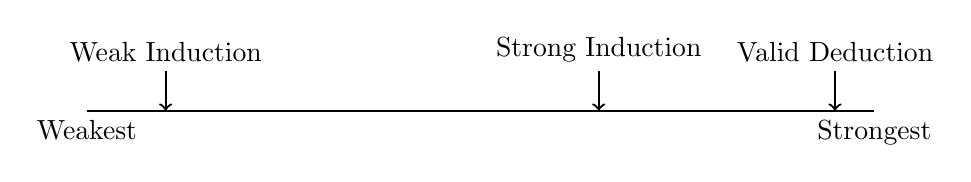
\begin{tikzpicture}
\draw[thick] (0,0) -- (10,0); % Strength continuum line
\node[below] at (0,0) {Weakest};
\node[below] at (10,0) {Strongest};
\draw[thick, ->] (1,0.5) -- (1,0); % Weak induction marker
\node[above] at (1,0.5) {Weak Induction};
\draw[thick, ->] (6.5,0.5) -- (6.5,0); % Strong induction marker
\node[above] at (6.5,0.5) {Strong Induction};
\draw[thick, ->] (9.5,0.5) -- (9.5,0); % Deduction marker
\node[above] at (9.5,0.5) {Valid Deduction};


\end{tikzpicture}
\end{frame}


\begin{frame}
\frametitle{13. Why Distinguishing Argument Forms Matters}
\begin{itemize}
\item Different argument forms serve different purposes in reasoning and communication.
\item The appropriate standard of evaluation depends on the argument's intended form.
\item Misidentifying an argument's form can lead to unfair criticism or unwarranted acceptance.
\item Some contexts (science, law, mathematics) require specific argument forms.

\end{itemize}

\begin{alertblock}{Common Mismatch Errors}
\begin{itemize}
\item Expecting deductive certainty from inductive arguments
\item Treating deductive arguments as merely probable
\item Accepting weak induction as if it were strong
\item Failing to recognize when certainty is impossible
\end{itemize}

\end{alertblock}
\end{frame}

\begin{frame}
\frametitle{14. Characteristics of Valid Deductive Arguments}
\begin{itemize}
\item \textbf{Necessity}: The conclusion must follow from the premises with absolute certainty.
\item \textbf{Truth preservation}: If premises are true, the conclusion cannot be false.
\item \textbf{No new information}: The conclusion only contains information implicit in the premises.
\item \textbf{Form determines validity}: The structure, not content, determines if an argument is valid.
\end{itemize}

\begin{block}{Testing for Validity}
A deductive argument is valid if and only if:
\begin{enumerate}
\item It is impossible for all premises to be true while the conclusion is false
\item The negation of the conclusion contradicts the premises
\item The conclusion is a logical consequence of the premises
\end{enumerate}
\end{block}
\end{frame}

\begin{frame}
\frametitle{15. Modus Ponens: "If P then Q, P, therefore Q"}
\begin{itemize}
\item \textbf{Modus Ponens} (affirming the antecedent) is a fundamental valid argument pattern.
\item Structure: If P then Q; P is true; Therefore, Q must be true.
\item The first premise establishes a conditional relationship; the second affirms the condition.
\item This form appears frequently in everyday reasoning and scientific thinking.
\end{itemize}

\begin{example}
\textbf{Modus Ponens in Action:}

P1: If it is raining, then the ground is wet.
P2: It is raining.
C: Therefore, the ground is wet.

\textit{Logical Form:} If P → Q; P; Therefore, Q
\end{example}
\end{frame}

\begin{frame}
\frametitle{16. Modus Tollens: "If P then Q, not Q, therefore not P"}
\begin{itemize}
\item \textbf{Modus Tollens} (denying the consequent) is another fundamental valid pattern.
\item Structure: If P then Q; Q is false; Therefore, P must be false.
\item This form uses the contrapositive relationship: if P→Q then ¬Q→¬P.
\item Modus Tollens is central to falsification in scientific reasoning.
\end{itemize}

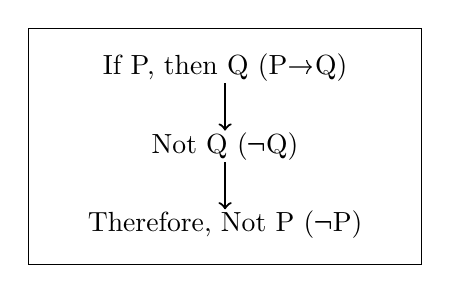
\begin{tikzpicture}
\draw (0,0) rectangle (5,3);
\node at (2.5,2.5) {If P, then Q (P→Q)};
\draw[thick, ->] (2.5,2.3) -- (2.5,1.7);
\node at (2.5,1.5) {Not Q (¬Q)};
\draw[thick, ->] (2.5,1.3) -- (2.5,0.7);
\node at (2.5,0.5) {Therefore, Not P (¬P)};


\end{tikzpicture}
\end{frame}


\begin{frame}
\frametitle{17. Hypothetical Syllogism: "If P then Q, if Q then R, therefore if P then R"}
\begin{itemize}
\item \textbf{Hypothetical syllogism} connects conditional statements in a chain.
\item New symbol: \newlogicalsymbol{$R$}{A third statement variable}
\item Structure: If $P \rightarrow Q$; If $Q \rightarrow R$; Therefore, if $P \rightarrow R$.
\item This pattern allows us to derive new conditional relationships transitively.
\item It demonstrates how valid arguments can combine to create new valid arguments.
\end{itemize}

\begin{example}
\textbf{Hypothetical Syllogism Example:}

P1: If it rains, the soccer match will be canceled. ($P \rightarrow Q$) \\
P2: If the soccer match is canceled, we will go to the movies. ($Q \rightarrow R$) \\
C: Therefore, if it rains, we will go to the movies. ($P \rightarrow R$) \\

\end{example}
\end{frame}

\begin{frame}
\frametitle{18. Disjunctive Syllogism: "P or Q, not P, therefore Q"}
\begin{itemize}
\item \textbf{Disjunctive syllogism} eliminates one option from an "either-or" scenario.
\item New symbol: \newlogicalsymbol{$P \lor Q$}{P or Q (disjunction)}
\item Structure: $P \lor Q$ is true; $\neg P$ is true; Therefore, $Q$ must be true.
\item This form assumes the disjunction is inclusive (at least one must be true).
\item It's useful for narrowing down possibilities through elimination.
\end{itemize}

\begin{block}{Key Requirements}
For a disjunctive syllogism to be valid:
\begin{itemize}
\item The disjunction must be exhaustive (covers all possibilities)
\item The eliminated option must be definitively ruled out
\item The disjunction is assumed to be true (at least one option must be true)
\end{itemize}

\end{block}
\end{frame}

\begin{frame}
\frametitle{19. Recognizing Valid Arguments in Everyday Language}
\begin{itemize}
\item Valid argument forms often appear in natural language without formal notation.
\item Key conditional phrases include "if...then," "when," "unless," and "only if."
\item Disjunctions appear as "either...or," "unless," and "at least one of these."
\item Negations may be expressed as "not," "never," "none," or other negative terms.
\end{itemize}

\begin{table}
\scriptsize
\begin{tabular}{|p{3cm}|p{7cm}|}
\hline
\textbf{Logical Form} & \textbf{Natural Language Example} \\
\hline
Modus Ponens ($P \rightarrow Q$; $P$; $\therefore Q$) & "Since it's raining, and rain makes things wet, the ground must be wet." \\
\hline
Modus Tollens ($P \rightarrow Q$; $\neg Q$; $\therefore \neg P$) & "The ground isn't wet, so it can't be raining." \\
\hline
Hypothetical ($P \rightarrow Q$; $Q \rightarrow R$; $\therefore P \rightarrow R$) & "If you study, you'll pass. If you pass, you'll graduate. So if you study, you'll graduate." \\
\hline
Disjunctive ($P \lor Q$; $\neg P$; $\therefore Q$) & "It's either in my purse or my car. It's not in my purse, so it must be in my car." \\
\hline
\end{tabular}
\end{table}
\end{frame}

\begin{frame}
\frametitle{20. What Makes a Fallacy "Formal"?}
\begin{itemize}
\item A \textbf{formal fallacy} is an error in the logical structure of an argument.
\item Formal fallacies make arguments invalid regardless of the content of the premises.
\item They involve incorrect patterns of reasoning that can be identified by their form alone.
\item Even arguments with true premises and true conclusions can be invalid due to formal fallacies.
\end{itemize}

\begin{table}
\centering
\begin{tabular}{|c|c|}
\hline
\textbf{Valid Forms} & \textbf{Invalid Forms (Fallacies)} \\
\hline
If $P \rightarrow Q$; $P$; Therefore $Q$ & If $P \rightarrow Q$; $Q$; Therefore $P$ \\
If $P \rightarrow Q$; $\neg Q$; Therefore $\neg P$ & If $P \rightarrow Q$; $\neg P$; Therefore $\neg Q$ \\
$P \lor Q$; $\neg P$; Therefore $Q$ & $P \lor Q$; $P$; Therefore $\neg Q$ \\
\hline
\end{tabular}
\caption{Comparison of Valid and Invalid Argument Forms}
\end{table}
\end{frame}

\begin{frame}
\frametitle{21. Affirming the Consequent: "If P then Q, Q, therefore P"}
\begin{itemize}
\item \textbf{Affirming the consequent} is an invalid argument form that confuses necessity with sufficiency.
\item Structure: If P then Q; Q is true; Therefore, P must be true.
\item This pattern wrongly assumes that if P leads to Q, then Q must have been caused by P.
\item The fallacy ignores that Q could have multiple possible causes besides P.
\end{itemize}

\begin{example}
\textbf{Affirming the Consequent Example:}

P1: If it is raining, then the ground is wet.
P2: The ground is wet.
C: Therefore, it is raining.

\textit{Why invalid:} The ground could be wet for other reasons (sprinklers, spilled water, etc.).
\end{example}
\end{frame}

\begin{frame}
\frametitle{22. Denying the Antecedent: "If P then Q, not P, therefore not Q"}
\begin{itemize}
\item \textbf{Denying the antecedent} is an invalid argument form that misunderstands conditional logic.
\item Structure: If P then Q; P is false; Therefore, Q must be false.
\item This pattern wrongly assumes that P is the only way to produce Q.
\item The fallacy fails to recognize that Q might occur for reasons other than P.
\end{itemize}

\begin{block}{Why This Form Is Invalid}
\begin{itemize}
\item The statement "If P then Q" only tells us what happens when P is true
\item It tells us nothing about what happens when P is false
\item When P is false, Q could still be true for other reasons
\item The relationship is one-directional unless explicitly stated otherwise
\end{itemize}
\end{block}
\end{frame}

\begin{frame}
\frametitle{23. The Fallacy of the Undistributed Middle}
\begin{itemize}
\item The \textbf{fallacy of the undistributed middle} occurs in categorical syllogisms.
\item Structure: All A are B; All C are B; Therefore, all A are C.
\item This pattern incorrectly assumes that because A and C share a common property B, they are the same.
\item The fallacy ignores that B could be a broad category containing distinct subcategories.
\end{itemize}

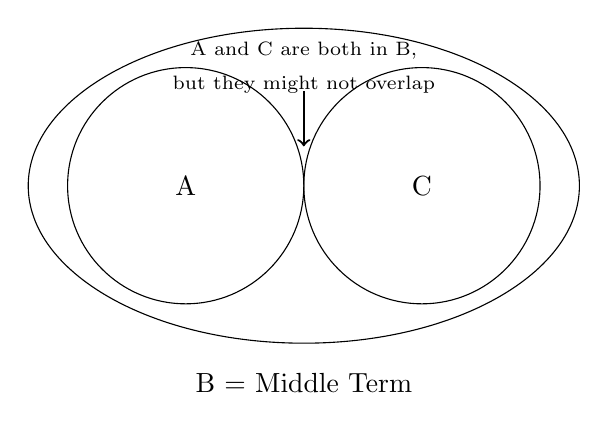
\begin{tikzpicture}
% Venn diagram showing undistributed middle
\draw (0,0) circle (1.5cm); % Circle A
\draw (3,0) circle (1.5cm); % Circle C
\draw (1.5,0) ellipse (3.5cm and 2cm); % Circle B containing both A and C
\node at (0,0) {A};
\node at (3,0) {C};
\node at (1.5,-2.5) {B = Middle Term};
\node[align=center] at (1.5,1.5) {\scriptsize A and C are both in B,\\ \scriptsize but they might not overlap};
\draw[->, thick] (1.5,1.2) -- (1.5,0.5);
\end{tikzpicture}
\end{frame}

\begin{frame}
\frametitle{24. How to Spot Formal Fallacies in Real Arguments}
\begin{itemize}
\item Convert the argument to standard form to identify its logical structure.
\item Look for conditional statements and check how they're used in the reasoning.
\item Examine the relationship between terms in categorical statements.
\item Test the argument by creating a counterexample with true premises and a false conclusion.
\end{itemize}

\begin{alertblock}{Common Warning Signs}
Be suspicious of arguments that:
\begin{itemize}
\item Conclude "Therefore A" when A appears as a sufficient condition for something
\item Conclude "Therefore not B" when the absence of a sufficient condition is noted
\item Claim two things are the same because they share a common property
\item Cannot be diagrammed coherently using logical notation
\end{itemize}
\end{alertblock}
\end{frame}

\begin{frame}
\frametitle{25. Characteristics of Strong Inductive Arguments}
\begin{itemize}
\item \textbf{Inductive arguments} move from specific evidence to general or probable conclusions.
\item A \textbf{strong inductive argument} provides good but not conclusive support for its conclusion.
\item The strength of induction is a matter of degree, not an all-or-nothing quality.
\item Strong induction depends on the quality, quantity, and relevance of evidence.
\end{itemize}

\begin{block}{Evaluating Inductive Strength}
An inductive argument is stronger when:
\begin{itemize}
\item The conclusion follows with higher probability
\item The evidence is more comprehensive and representative
\item Alternative explanations have been considered and addressed
\item The inductive leap (from evidence to conclusion) is smaller
\end{itemize}
\end{block}
\end{frame}

\begin{frame}
\frametitle{26. Inductive Generalizations: From Sample to Population}
\begin{itemize}
\item \textbf{Inductive generalization} extends observations about a sample to an entire population.
\item Structure: X\% of observed A's have property B; Therefore, X\% of all A's have property B.
\item The strength depends on sample size, randomness, and representativeness.
\item This form is fundamental to scientific research and statistical reasoning.
\end{itemize}

\begin{table}
\scriptsize
\begin{tabular}{|l|l|}
\hline
\textbf{Factor} & \textbf{Impact on Strength} \\
\hline
Sample Size & Larger samples typically provide stronger support \\
\hline
Randomness & Random samples reduce selection bias \\
\hline
Representativeness & Sample should reflect population characteristics \\
\hline
Variability & Less variability in population strengthens generalization \\
\hline
\end{tabular}
\end{table}
\end{frame}

\begin{frame}
\frametitle{27. Statistical Syllogisms: From Population to Individual}
\begin{itemize}
\item \textbf{Statistical syllogisms} apply population statistics to make judgments about individuals.
\item Structure: X\% of A's are B; This is an A; Therefore, this is probably a B.
\item The probability assigned to the conclusion should match the statistical frequency.
\item Strength increases as the percentage approaches 100\% (or 0\% for negative cases).
\end{itemize}

\begin{example}
\scriptsize
\textbf{Statistical Syllogism Example:}\\

P1: 90\% of flight departures from this airport are on time.\\
P2: Flight 372 is departing from this airport.\\
C: Therefore, Flight 372 will probably (with 90\% probability) be on time.\\

\textit{Note:} Strength depends on the statistical percentage and absence of defeaters.
\end{example}
\end{frame}

\begin{frame}
\frametitle{28. Arguments from Analogy: When Similarities Matter}
\begin{itemize}
\item \textbf{Arguments from analogy} reason that similar cases will have similar outcomes.
\item Structure: A and B share properties P, Q, R; A has property S; Therefore, B probably has property S.
\item Strength depends on relevance and number of similarities between the compared cases.
\item These arguments are common in legal reasoning, ethics, and scientific discovery.
\end{itemize}

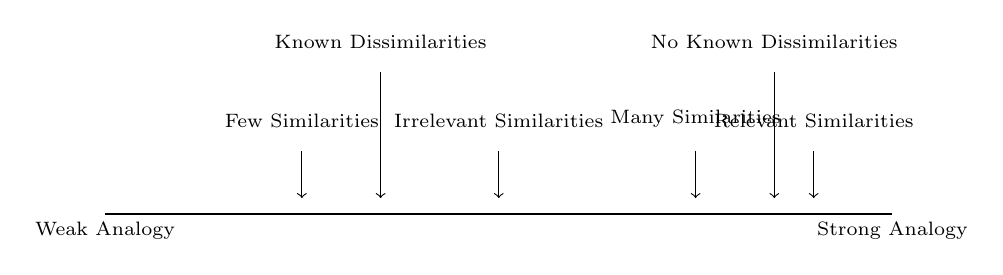
\begin{tikzpicture}
\scriptsize
% Analogy strength diagram
\draw[thick] (0,0) -- (10,0); % Strength continuum line
\node[below] at (0,0) {Weak Analogy};
\node[below] at (10,0) {Strong Analogy};

% Factors affecting strength
\node[above] at (2.5,1) {Few Similarities};
\draw[->] (2.5,0.8) -- (2.5,0.2);

\node[above] at (5,1) {Irrelevant Similarities};
\draw[->] (5,0.8) -- (5,0.2);

\node[above] at (7.5,1) {Many Similarities};
\draw[->] (7.5,0.8) -- (7.5,0.2);

\node[above] at (9,1) {Relevant Similarities};
\draw[->] (9,0.8) -- (9,0.2);

\node[above] at (3.5,2) {Known Dissimilarities};
\draw[->] (3.5,1.8) -- (3.5,0.2);

\node[above] at (8.5,2) {No Known Dissimilarities};
\draw[->] (8.5,1.8) -- (8.5,0.2);
\end{tikzpicture}
\end{frame}


\begin{frame}
\frametitle{29. Causal Arguments: Establishing Cause and Effect}
\begin{itemize}
\item \textbf{Causal arguments} attempt to establish that one event causes another.
\item Strong causal arguments require temporal precedence, correlation, and ruling out alternative causes.
\item Scientific methods like controlled experiments help strengthen causal claims.
\item Causal reasoning is fundamental to explaining events and making predictions.
\end{itemize}

\begin{block}{Mill's Methods for Establishing Causation}
\scriptsize
\begin{itemize}
\item \textbf{Method of Agreement:} If multiple instances of a phenomenon have one factor in common, that factor may be the cause
\item \textbf{Method of Difference:} If two situations differ only in one factor and one outcome, that factor may cause the outcome
\item \textbf{Method of Concomitant Variation:} If variations in one factor correlate with variations in another, they may be causally related
\end{itemize}
\end{block}
\end{frame}

\begin{frame}
\frametitle{30. When Inductive Arguments Fall Short}
\begin{itemize}
\item \textbf{Weak inductive arguments} provide insufficient support for their conclusions.
\item The probability that the conclusion follows from the premises is low.
\item Weak arguments contain significant gaps, oversights, or logical leaps.
\item They may still be useful starting points, but require additional evidence or reasoning.
\end{itemize}

\begin{table}
\scriptsize
\begin{tabular}{|l|l|}
\hline
\textbf{Strong Induction} & \textbf{Weak Induction} \\
\hline
Large, representative samples & Small, biased samples \\
\hline
Relevant similarities in analogies & Superficial similarities in analogies \\
\hline
Multiple causes considered & Alternative causes ignored \\
\hline
Moderate claims relative to evidence & Sweeping claims beyond evidence \\
\hline
\end{tabular}
\end{table}
\end{frame}

\begin{frame}
\frametitle{31. Sample Size Problems: Too Few Examples}
\begin{itemize}
\item \textbf{Small sample size} undermines the reliability of generalizations.
\item Single examples or anecdotes rarely justify broad conclusions about populations.
\item The margin of error increases as sample size decreases.
\item Random variation can easily be mistaken for meaningful patterns in small samples.
\end{itemize}

\begin{example}
\textbf{Sample Size Problem Example:}

"I know three people who got headaches after taking this medication, so it must commonly cause headaches."

\textit{Why weak:} Three cases is too small a sample to determine the actual frequency of side effects in the broader population. The observed cases might not be representative.
\end{example}
\end{frame}


\begin{frame}
\frametitle{32. Representativeness Issues: Biased Samples}
\begin{itemize}
\item A \textbf{biased sample} contains systematic errors that undermine generalization.
\item Common biases include self-selection, convenience sampling, and confirmation bias.
\item Even large samples can be unreliable if they aren't representative of the target population.
\item Identifying and correcting for bias is essential in scientific research and polling.
\end{itemize}

\begin{alertblock}{Examples of Biased Samples}
\scriptsize
\begin{itemize}
\item \textbf{Self-Selection Bias:} Surveying only people who volunteer to participate, which may not represent the general population.
\item \textbf{Convenience Sampling:} Using a sample that is easy to access, such as surveying students in a single classroom to represent all students.
\item \textbf{Confirmation Bias:} Selecting data that supports a preconceived notion while ignoring data that contradicts it.
\item \textbf{Survivorship Bias:} Focusing on successful cases while overlooking those that failed, such as studying only successful companies to understand business practices.
\end{itemize}
\end{alertblock}
\end{frame}


\begin{frame}
\frametitle{33. Correlation vs. Causation Distinctions}
\begin{itemize}
    \item \textbf{Correlation} means two variables tend to occur together or change together.
    \item \textbf{Causation} means one variable directly influences or produces another.
    \item Correlation alone is insufficient to establish a causal relationship.
    \item Alternative explanations for correlation include coincidence, common cause, and reverse causation.
\end{itemize}

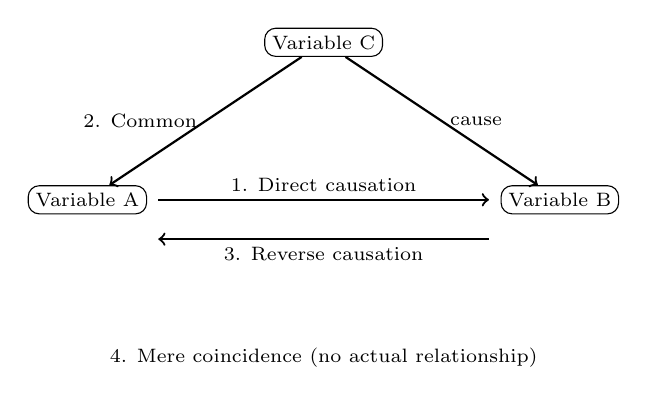
\begin{tikzpicture}
\scriptsize
% Possible relationships between correlated variables
\node[draw, rectangle, rounded corners] (A) at (0,0) {Variable A};
\node[draw, rectangle, rounded corners] (B) at (6,0) {Variable B};

% Direct causation
\draw[thick, ->] (0.9,0) -- (5.1,0) node[midway, above] {1. Direct causation};

% Common cause
\node[draw, rectangle, rounded corners] (C) at (3,2) {Variable C};
\draw[thick, ->] (C) -- (A) node[midway, left] {2. Common};
\draw[thick, ->] (C) -- (B) node[midway, right] {cause};

% Reverse causation
\draw[thick, ->] (5.1,-0.5) -- (0.9,-0.5) node[midway, below] {3. Reverse causation};

% Coincidence
\node at (3,-2) {4. Mere coincidence (no actual relationship)};
\end{tikzpicture}
\end{frame}

\begin{frame}
\frametitle{34. Hasty Generalization: Jumping to Conclusions}
\begin{itemize}
    \item \textbf{Hasty generalization} occurs when a conclusion is drawn from insufficient evidence.
    \item This fallacy involves making a broad claim based on too few examples or atypical cases.
    \item The error lies in treating a small or unrepresentative sample as adequate support.
    \item Hasty generalizations often reflect cognitive biases like the availability heuristic.
\end{itemize}

\begin{example}
\textbf{Hasty Generalization Examples:}
\scriptsize

"My neighbor's electric car had battery problems, so electric cars are unreliable." \\

"I got food poisoning at a Mexican restaurant once, so Mexican food is unsafe." \\

\textit{Why fallacious:} Drawing broad conclusions about entire categories based on single instances or very limited experience.
\end{example}
\end{frame}

\begin{frame}
\frametitle{35. Post Hoc Ergo Propter Hoc: After This, Therefore Because of This}
\begin{itemize}
    \item \textbf{Post hoc ergo propter hoc} assumes that if B follows A, A must have caused B.
    \item This fallacy mistakes temporal sequence for causal relationship.
    \item The error lies in ignoring other potential causes or coincidental timing.
    \item This fallacy is common in everyday reasoning, superstitions, and pseudoscience.
\end{itemize}

\begin{block}{Avoiding the Post Hoc Fallacy}
    To avoid this fallacy, ask:
    \begin{itemize}
        \item Could the timing be coincidental?
        \item Are there other plausible explanations?
        \item Is there a logical mechanism connecting cause and effect?
        \item Would controlled studies confirm the causal relationship?
    \end{itemize}
\end{block}
\end{frame}

\begin{frame}
\frametitle{36. Appeal to Unqualified Authority: When Expert Opinion Isn't Expert}
\begin{itemize}
    \item \textbf{Appeal to unqualified authority} occurs when citing someone who lacks relevant expertise.
    \item The fallacy treats expertise in one domain as transferable to unrelated domains.
    \item The error lies in confusing fame, status, or credentials with subject-specific knowledge.
    \item Even genuine experts can be wrong, especially outside their field of expertise.
\end{itemize}

\begin{table}
    \scriptsize
\begin{tabular}{|l|l|}
\hline
\textbf{Valid Expert Appeal} & \textbf{Appeal to Unqualified Authority} \\
\hline
Expert has relevant qualifications & Person lacks relevant expertise \\
\hline
Expert represents consensus view & Opinion contradicts consensus \\
\hline
Expert provides reasoning/evidence & Authority simply states conclusion \\
\hline
Field has established standards & Field lacks scientific standards \\
\hline
\end{tabular}
\end{table}
\end{frame}

\begin{frame}
    \frametitle{37. Appeal to Ignorance: Absence of Evidence Isn't Evidence of Absence}
    \begin{itemize}
        \item \textbf{Appeal to ignorance} claims something is true because it hasn't been proven false (or vice versa).
        \item This fallacy shifts the burden of proof improperly.
        \item The error lies in treating lack of evidence as evidence itself.
        \item Special contexts like legal presumptions ("innocent until proven guilty") are exceptions, not appeals to ignorance.
    \end{itemize}
    
    \begin{example}
    \textbf{Appeal to Ignorance Examples:}
    
    "Scientists haven't proven that this herb doesn't cure cancer, so it must work."
    
    "No one has proven that ghosts exist, so they must not exist."
    
    \textit{Why fallacious:} Both examples improperly treat absence of evidence as positive evidence for the contrary position.
    \end{example}
    \end{frame}
    
    \begin{frame}
    \frametitle{38. Slippery Slope Fallacy: When Small Steps Don't Lead to Disaster}
    \begin{itemize}
        \item The \textbf{slippery slope fallacy} claims that a small action will inevitably lead to extreme consequences.
        \item This fallacy exaggerates the likelihood of a chain of events without adequate justification.
        \item The error lies in assuming each step must follow without allowing for intervention or stabilization.
        \item Not all slippery slope arguments are fallacious—some chains of events are genuinely likely.
    \end{itemize}

    \begin{alertblock}{Examples of Slippery Slope Fallacy}
        \scriptsize
    \begin{itemize}
        \item "If we allow students to redo assignments, soon they'll expect to retake entire courses."
        \item "If we ban smoking in public places, eventually the government will ban all personal freedoms."
        \item "If we legalize marijuana, it will lead to the legalization of all drugs."
        \item "If we start regulating social media, it will lead to complete government control over the internet."
    \end{itemize}
    \end{alertblock}
    
\end{frame}
    
    \begin{frame}
    \frametitle{39. The Texas Sharpshooter Fallacy: Cherry-Picking Evidence}
    \begin{itemize}
        \item The \textbf{Texas Sharpshooter Fallacy} involves cherry-picking data to fit a predetermined conclusion.
        \item This fallacy gets its name from a shooter who fires at a wall, then draws a target around the cluster of hits.
        \item The error lies in ignoring data that contradicts the desired pattern or selectively defining patterns.
        \item This fallacy is common in confirmation bias, conspiracy theories, and pseudoscience.
    \end{itemize}
    
    \begin{block}{How to Avoid Cherry-Picking}
        To avoid this fallacy:
        \begin{itemize}
            \item Define criteria and predictions before examining data
            \item Consider all relevant evidence, not just confirming examples
            \item Ask what evidence would disprove your hypothesis
            \item Use statistical methods that account for multiple comparisons
        \end{itemize}
    \end{block}
    \end{frame}
    
    \begin{frame}
    \frametitle{40. The Gambler's Fallacy: Misunderstanding Probability and Independence}
    \begin{itemize}
        \item The \textbf{Gambler's Fallacy} assumes that independent random events are influenced by past outcomes.
        \item This fallacy leads people to believe that a string of one outcome increases chances of the opposite.
        \item The error lies in failing to understand statistical independence in random processes.
        \item Each independent trial has the same probability regardless of previous results.
    \end{itemize}
    
    \begin{example}
    \textbf{Gambler's Fallacy Example:}
    
    "The roulette wheel has landed on black six times in a row. Red is definitely due to come up next!"
    
    \textit{Why fallacious:} The roulette wheel has no "memory" of previous spins. Each spin is an independent event with the same probability distribution. Past results do not influence future outcomes in truly random processes.
    \end{example}
    \end{frame}

\end{document}